\documentclass{article}
\usepackage[a4paper, margin=1in]{geometry}
\usepackage{float}
\usepackage{graphicx} % Required for inserting images
\usepackage{amsmath}
\usepackage{amsfonts}
\usepackage[colorlinks=true, linkcolor=black]{hyperref}
\usepackage{cleveref}
\usepackage{hyperref}
\usepackage{float}
\usepackage[justification=centering]{caption}
\usepackage[backend=bibtex]{biblatex}
\addbibresource{references.bib}
\title{A Physics-Informed Neural Network (PINN) Based Surrogate Model to Study Gravitational Collapse in Self-Gravitating Molecular Clouds}
\author{
  Tirthankar De \\
  Indian Institute of Technology Roorkee \\
  \and
  \textbf{Supervisor:} Dr. Sayantan Auddy \\
  Fields Institute for Research in Mathematical Sciences, University of Toronto
}
\date{July 2025}

\begin{document}
\maketitle

\section{Introduction}
Modelling self-gravitating molecular clouds is fundamental to understanding cosmic structure formation, but simulating their non-linear dynamics is challenging. While traditional methods like Finite Difference (FD) have been used, they are limited by computational costs that scale exponentially with dimensionality, hindering long-term or high-resolution studies. Physics-Informed Neural Networks (PINNs) offer a promising solution. As shown by the Gravity-informed neural network (GRINN) \cite{auddy2023grinnphysicsinformedneuralnetwork} paper, PINNs provide a mesh-free framework that avoids the prohibitive scaling of FD methods and demonstrates superior stability. 

However, the practical application of PINNs is limited because they require time-consuming retraining for each new set of physical parameters. This hinders their development into efficient surrogate models capable of learning solutions across a continuous parameter space. This project takes the first step toward creating such a model for simulating the gravitational collapse of molecular clouds. 

We extend the GRINN framework to treat the initial perturbation strength as a learnable parameter, a method inspired by recent work on parameter-informed PINNs (${P^2INNs}$) \cite{cho2024parameterizedphysicsinformedneuralnetworks}. This allows a single, trained model to capture the dynamics of both stable and unstable systems, establishing a viable path toward powerful and efficient surrogate models for complex astrophysical simulations. 

\section{Hydrodynamic System}
Similar to the GRINN paper, we solve the system of isothermal self-gravitating hydrodynamics, which is of interest in the study of interstellar molecular clouds, the sites of current-day star formation. 
The behaviour of the interstellar gas is governed by a set of fundamental hydrodynamic equations. We solve the three-dimensional (3D) hydrodynamic equations including self-gravity to study the gravitational (or Jeans [24]) instability in star-forming molecular clouds. If $\rho$ and $\mathbf{v}$ are the gas density and velocity respectively we can express the governing equations as
\begin{equation}
    \partial_t \rho + \nabla \cdot (\rho \mathbf{v}) = 0
    \label{eq:1}
\end{equation}
\begin{equation}
    \rho \left[ \partial_t \mathbf{v} + (\mathbf{v} \cdot \nabla) \mathbf{v} \right] = -\nabla P + \rho \mathbf{g}
    \label{eq:2}
\end{equation}
\begin{equation}
    \nabla^2 \phi = 4 \pi G \rho
    \label{eq:3}
\end{equation}
Eqs.~\eqref{eq:1} to~\eqref{eq:3} are the equations of mass continuity, momentum, and self-gravity (the Poisson equation),
 respectively. The gravitational field $\mathbf{g} = -\nabla \phi$, where $\phi$ is the gravitational potential given in eq.~\hyperref[eq:3]{(3)} and $G$ is the gravitational constant. Here we apply sinusoidal perturbations to the background steady-state fluid and study the behaviour under the influence of self-gravity. 
In the project we consider both linear and non-linear initial sinusoidal perturbations. Linear perturbations are small amplitude ($< 0.1\rho_0$) waves while non-linear perturbations are large amplitude ($> 0.1\rho_0$) disturbances to the uniform background density $\rho_0$. This fluid system has known analytic solutions, letting us probe the effectiveness of the \textit{PINN} architecture introduced in the next section for solving the \textit{GHD} equations.

\begin{figure}[H]
     \centering
     \makebox[\textwidth][c]{%
     \includegraphics[width=1.1\linewidth]{architecture.png}
     }
    \caption{Schematic of PINN's architecture}
    \label{Architecture}
\end{figure}

\section{PINN architecture}
The core of our model is a modular design that separates the processing of physical parameters from the spatio-temporal coordinates. Our architecture is composed of three main components: a Parameter Embedding Network, a Coordinate Embedding Network, and a central Manifold Network .

\subsection{Parameter and Coordinate Encoding}

To effectively learn the system's behaviour across a range of initial conditions, the model first encodes the inputs into latent representations using two specialized subnetworks:

\subsubsection{Parameter Embedding Network}
This subnetwork is dedicated solely to processing the the perturbation strength $\rho_{1a}$, which is passed through a small multi-layer perceptron (MLP) consisting of two linear layers and a Tanh activation function. This network transforms the scalar parameter into a 32-dimensional latent vector, $\mathbf{h}_{param}$. This dedicated encoding allows the model to capture a rich, high-dimensional representation of how the perturbation strength influences the overall dynamics. 

\subsubsection{Input Embedding Network}
This subnetwork processes the spatio-temporal coordinates of the system. The spatial coordinate \textit{x} and time \textit{t} are concatenated and fed into a separate MLP. This network, composed of four linear layers and sinusoidal activation function Sin, produces a 64-dimensional feature vector, $\mathbf{h}_{coord}$, that represents the state of the system at a specific point in space and time.

\subsection{Manifold Network}
The latent vectors $\mathbf{h}_{param}$ and $\mathbf{h}_{coord}$ are concatenated to form a single 96-dimensional tensor. This tensor is then fed into the main "manifold network," which is responsible for approximating the final solution. This central network is a deep MLP consisting of six hidden layers, each with 96 neurons. Key features of this network include:
\begin{itemize}
    \item Sinusoidal Activations: The network exclusively uses the sine function as its activation. This choice is crucial for representing complex, high-frequency functions and their derivatives, which is essential for satisfying the governing PDEs of the physical system. Networks with sinusoidal activations are known for their ability to fit intricate signals.
    \item Residual Connection: A residual or "skip" connection is incorporated into the network, where the output of the first hidden layer is added to the output of the fourth hidden layer. This technique is known to improve training stability in deep networks by mitigating the vanishing gradient problem, ensuring that information from earlier layers can propagate more effectively through the model.
\end{itemize}

 The output of this deep network is then passed to a final linear layer that maps the internal representation to the physical quantities of interest: density and velocity, thus forming the solution $\mathbf{u}(\mathbf{x}, t; \boldsymbol{\rho_{1a}})$. The entire network is initialized using Xavier uniform initialization to promote stable and efficient training from the outset. By combining a modular ${P^2INN}$-inspired design with a deep sinusoidal network, this architecture is robustly designed to learn the complex relationship between initial conditions and the evolution of gravitational collapse.

 \section{Results}
 We quantitatively assess the model performance using the mismatch $\epsilon$ of the density, velocity or gravitational potential relative to the Linear Theory (LT) solution (for linear perturbations) and/or FD solution, where $\epsilon$ is defined by

 \begin{equation}
     \epsilon = \frac{2|(\rho, \mathbf{v}, \phi)_{GRINN} - (\rho, \mathbf{v}, \phi)_{FD/LT} |}{(\rho, \mathbf{v}, \phi)_{GRINN} + (\rho, \mathbf{v}, \phi)_{FD/LT}}
 \end{equation}
 \begin{figure}[H]
     \centering
     \makebox[\textwidth][c]{%
     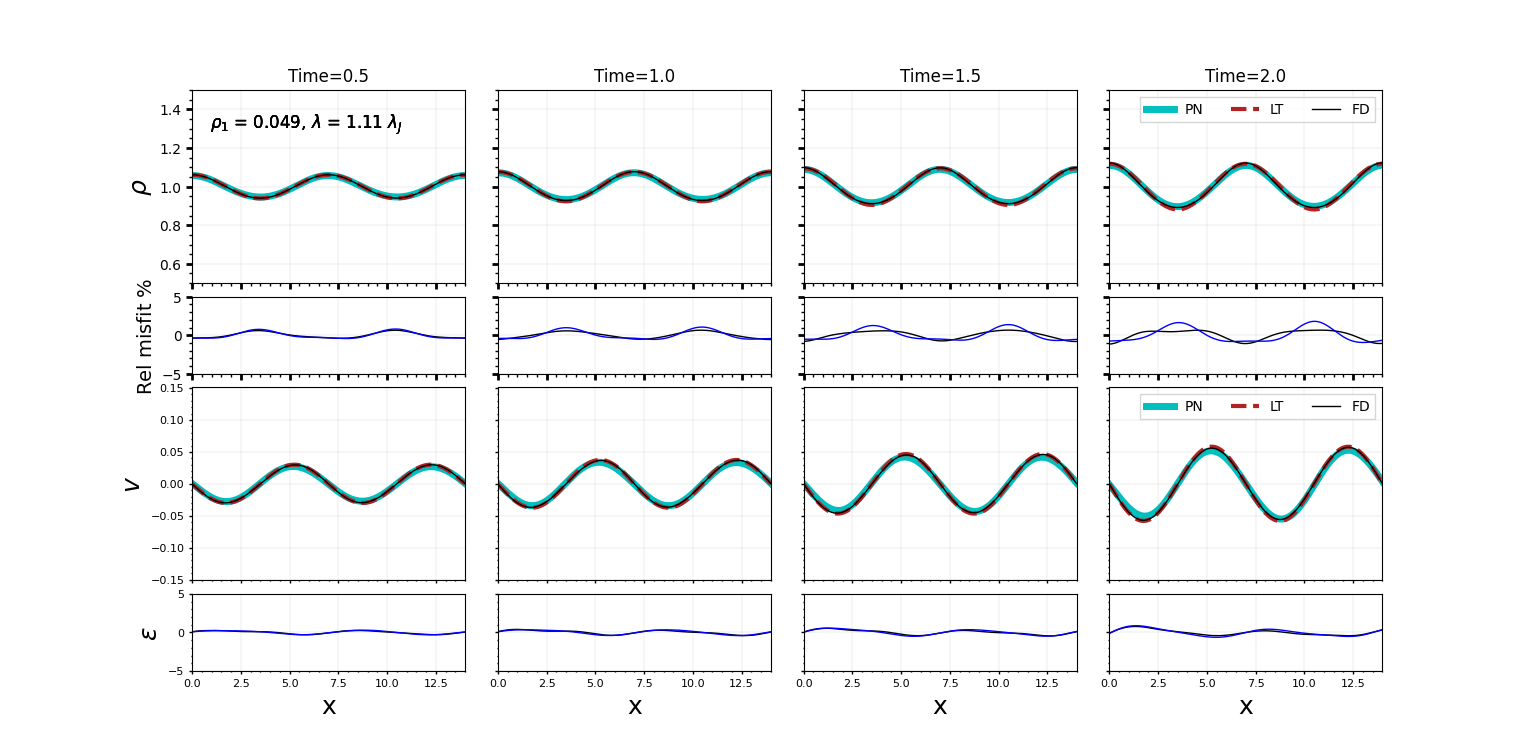
\includegraphics[width=0.9\linewidth]{Case 1/case 1 test value 2.png}
     }
     \caption{Density and velocity profiles at four times with mismatch; linear perturbation}
     \label{Figure 1}
 \end{figure}
\subsection{Growing linear perturbation with \texorpdfstring{$\lambda > \lambda_j$}{lambda > lambda\_j}}

Similar to the GRINN paper, we train our model on the equations ~\eqref{eq:1} to ~\eqref{eq:3} for initial conditions with a perturbation in density $\rho$ and 1D velocity amplitude $\mathbf{v}$ that corresponds to an individual mode under the LT:
\begin{equation}
    \rho(x, t = 0) = \rho_o + \rho_{1a}cos(k\cdot x)
\end{equation}
\begin{equation}
    v(x, t = 0) = v_{1a}sin(k\cdot x)
\end{equation}
where $v_{1a} = \frac{-\alpha}{k}\frac{\rho_{1a}}{\rho_o}$, $k$ is the wave vector and $\alpha = \sqrt{4\pi G\rho_o - {c_s}^2k^2}$. The difference in our case is that $\rho_{1a}$ is not fixed, but is instead a parameter learnt by our model.
We train our model with a set of $20$ random values of the perturbation strength within a range of $0.01$ and $0.08$, and the results for $\rho_{1a} = 0.049$ are shown in \autoref{Figure 1}. One thing to note is that the model is trained up to time $t = 1.5$, whereas the figure shows the solutions at $t = 2.0$ as well, showing the slight extrapolation ability of the network in the temporal domain. For the FD solution we choose Courant number to be $0.5$ and number of grid points $N = 1000$. One more interesting observation is that the velocity variation of the gas is $90^{\circ}$ out of phase with the density so that zero velocity coincides with the maximum velocity.

\begin{figure}[H]
     \centering
     \makebox[\textwidth][c]{%
     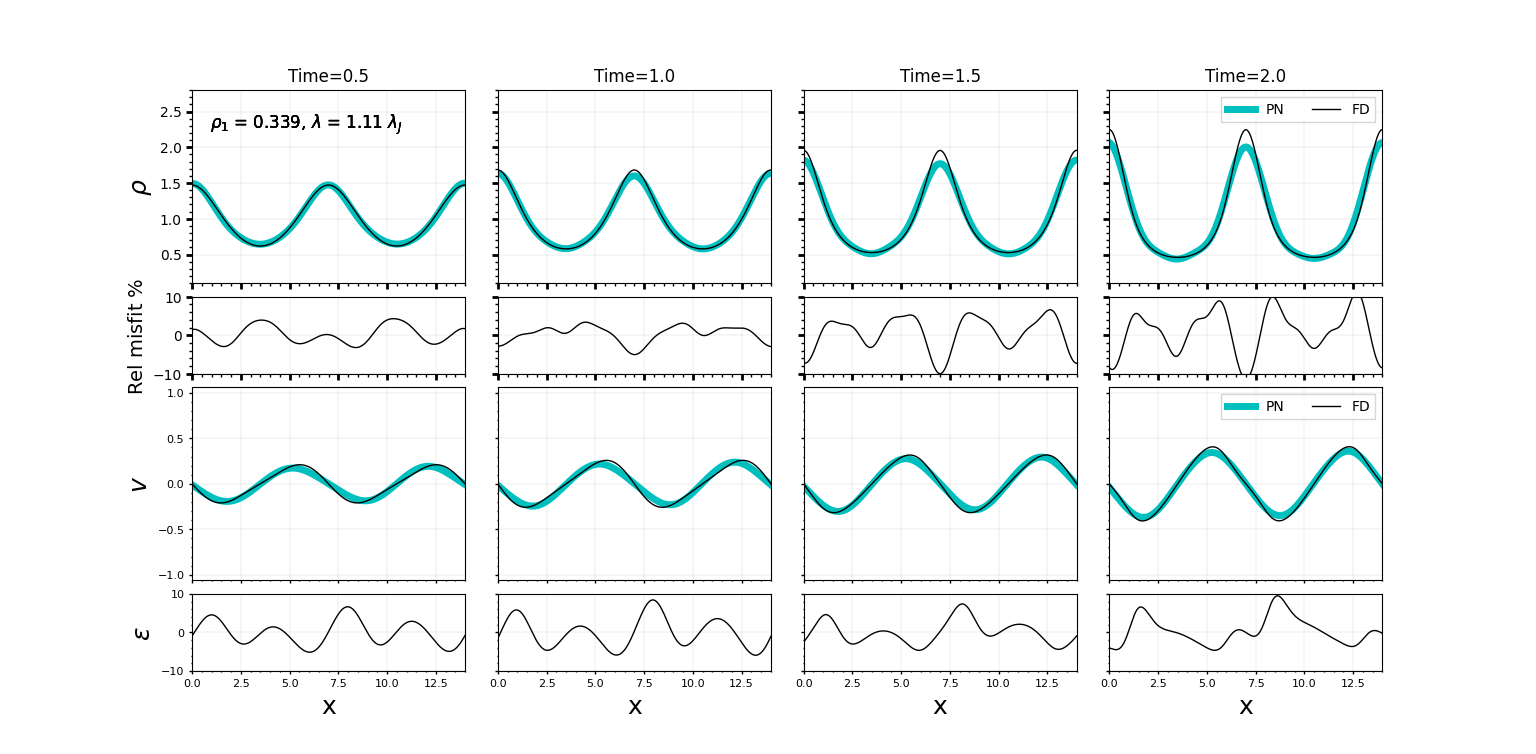
\includegraphics[width=0.9\linewidth]{Case 2/case 2 test value 2.png}
     }
    \caption{Density and velocity profiles at four times with mismatch; non-linear perturbation}
    \label{Figure 2}
\end{figure}

\subsection{Growing non-linear perturbation with \texorpdfstring{$\lambda > \lambda_j$}{lambda > lambda\_j}}
Next we examine the model performance on large amplitude, non-linear initial perturbations. We train the model on $20$ random values between $0.1$ and $0.8$, and the results for $\rho_{1a} = 0.339$ are shown in \autoref{Figure 2}. All other parameters remain the same as for linear case, except that to enhance stability of the FD solution, $N$ is increased to $8000$. Since the linear theory is invalid at such large amplitudes, we only compare results with FD solutions. We note that non-linear effects shift the maximum infall velocities toward the density peaks, leading to a slight asymmetry in the velocity profile that is evident in the solutions.

\begin{figure}[H]
     \centering
     \makebox[\textwidth][c]{%
     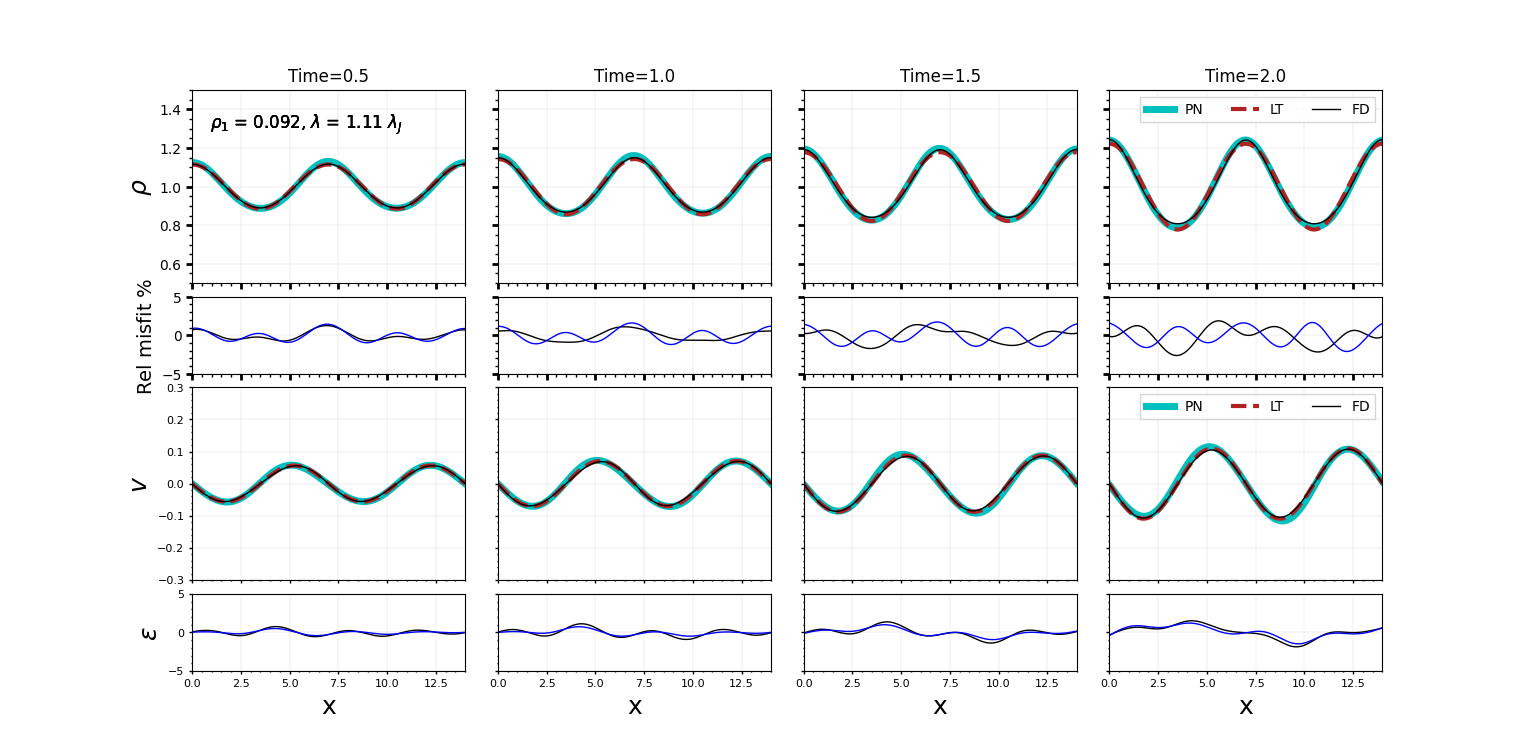
\includegraphics[width=0.9\linewidth]{Mixed case 1 and 2/mixed case value 1.png}
     }
    \caption{Density and velocity profiles near transition region with mismatch; linear perturbation}
    \label{Figure 3}
\end{figure}
\begin{figure}[H]
     \centering
     \makebox[\textwidth][c]{%
     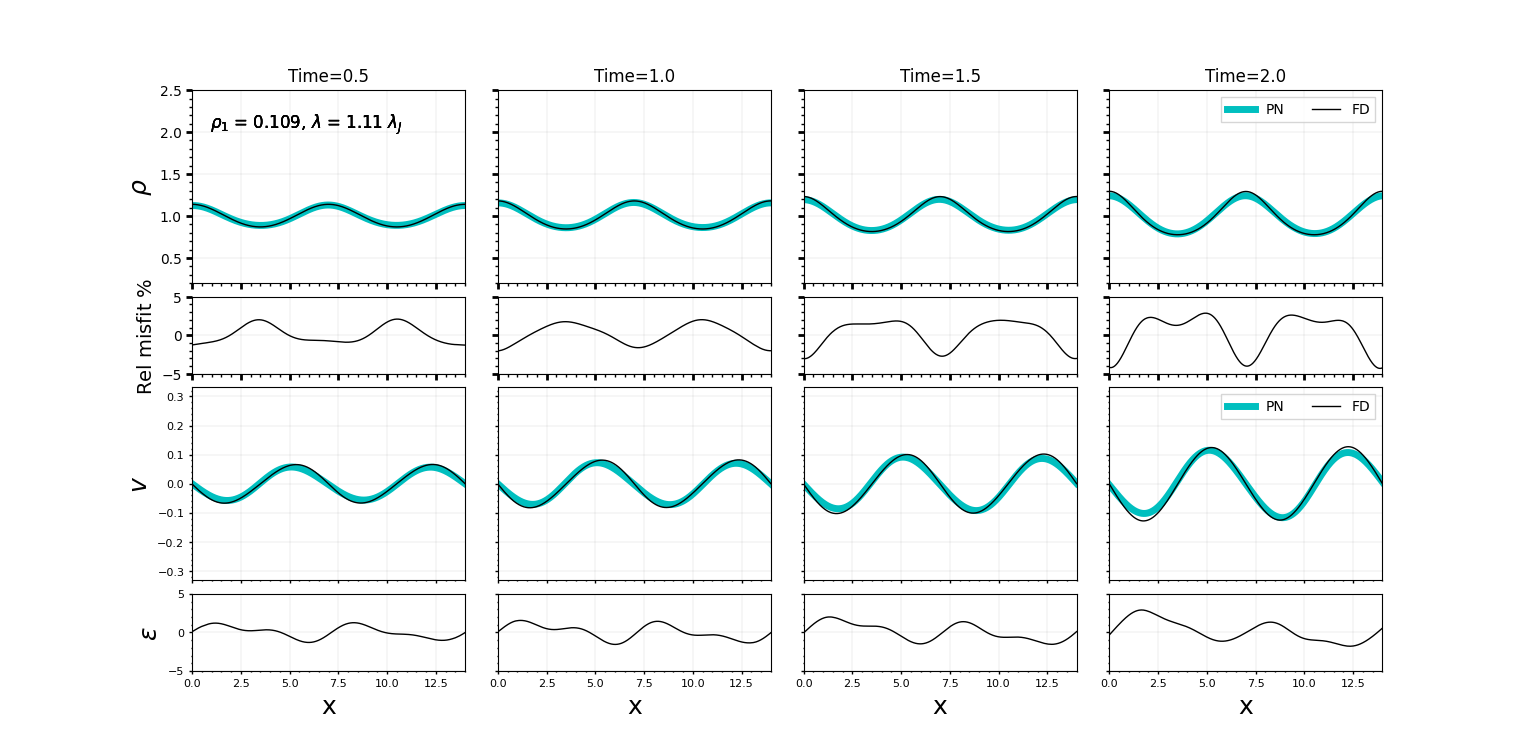
\includegraphics[width=0.9\linewidth]{Mixed case 1 and 2/mixed case value 3.png}
     }
    \caption{Density and velocity profiles near transition region with mismatch; non-linear perturbation}
    \label{Figure 4}
\end{figure}

\begin{figure}[H]
     \centering
     \makebox[\textwidth][c]{%
     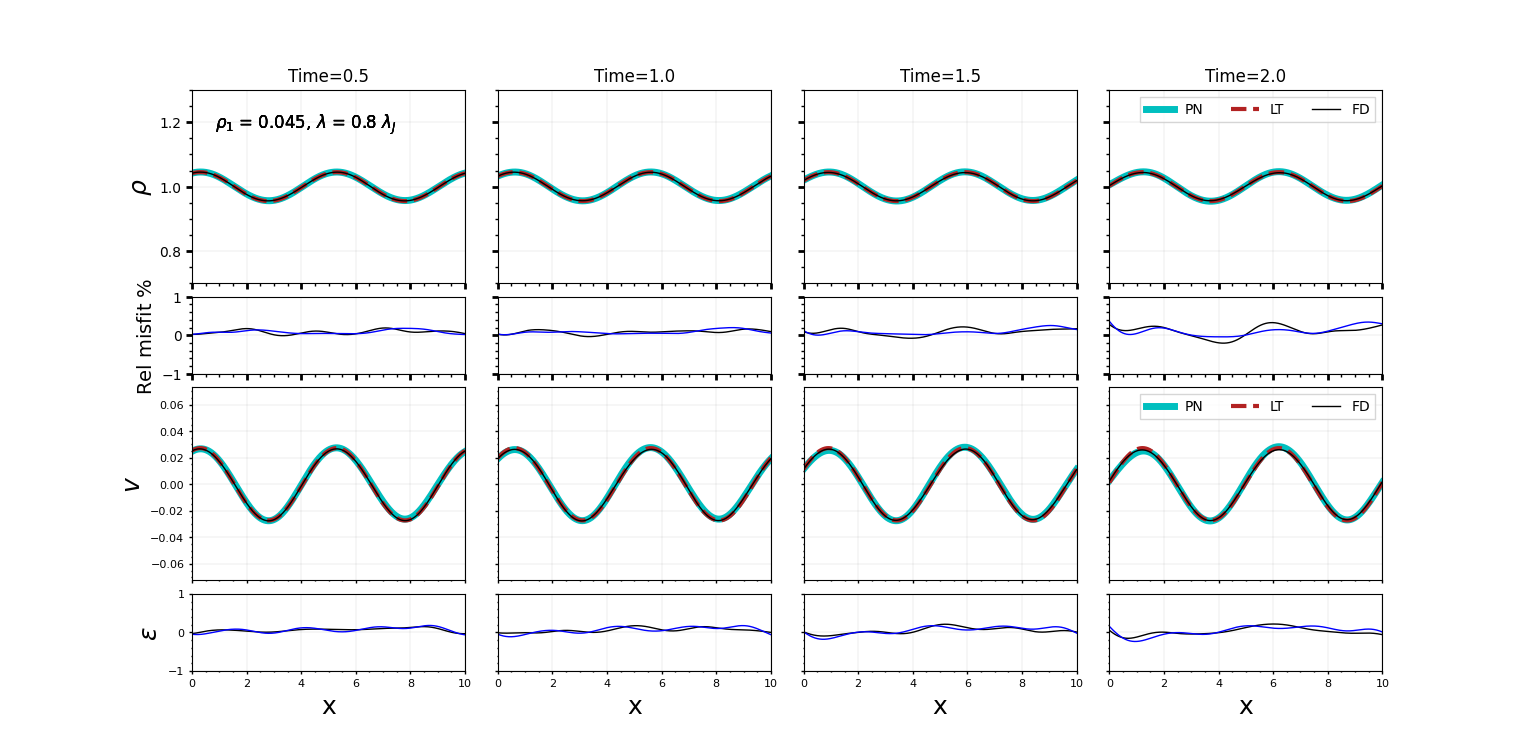
\includegraphics[width=0.9\linewidth]{Case 3/Case 3 value 2.png}
     }
    \caption{Density and velocity profiles for propagating linear perturbation}
    \label{Figure 5}
\end{figure}

\subsection{Transition region with \texorpdfstring{$\lambda > \lambda_j$}{lambda > lambda\_j}}

Next we examine a special case of the model's behaviour near the transition region. For this case we train the model on $20$ random values between $0.09$ and $0.11$, and the results for $\rho_{1a} = 0.092$ (linear perturbation) and $\rho_{1a} = 0.109$ (non-linear perturbation) are shown in \autoref{Figure 3} and \autoref{Figure 4} respectively. As can be seen, for both linear and non-linear values the model predictions agree to within $5\%$
of LT and/or FD solutions for the entire time interval.

\subsection{Propagating linear perturbation with \texorpdfstring{$\lambda < \lambda_j$}{lambda < lambda\_j}}

Finally we explore the model's performance on a propagating disturbance. For simplicity, we train the model on linear perturbations ($20$ random values between $0.01$ and $0.08$, and the results for $\rho_{1a} = 0.045$ is shown in \autoref{Figure 5}. As can be seen, the model predictions are within $1\%$ of LT and FD solutions.

\begin{figure}[H]
     \centering
     \makebox[\textwidth][c]{%
     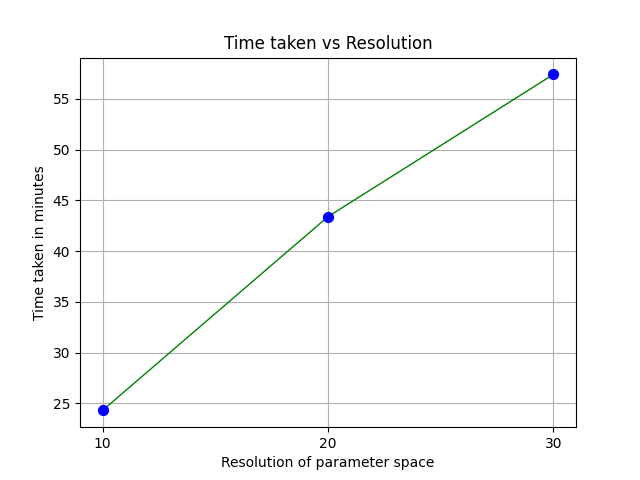
\includegraphics[width=0.7\linewidth]{Time vs Res.png}
     }
    \caption{Time taken for training across various resolutions of $\rho_{1a}$ space}
    \label{Figure 6}
\end{figure}

\section{Further insights and discussion}

Physics-informed neural networks like GRINN have opened promising new directions for solving astrophysical gas flow problems accurately in a time-efficient way. They can be built on top of publicly-available neural network modules like TensorFlow and PyTorch, making them easy to develop and maintain. Since these public modules are designed to run on GPUs, PINN-based
solvers can be implemented on GPU clusters with little effort, easing further enhancements in efficiency.
However current PINN models suffer the problem that whenever solutions to a new set of parameters are required, the model has to be re-trained. Such repetitive training from scratch limits PINNs to be used in research or industry. Our model solves this problem by having a single PINN learn the solutions of the PDEs across a wide parameter space.
In the following sections we discuss some of the pros and cons of the current framework.

\subsection{Computational cost variation with increase in parameter space resolution}

Here we compare the training cost of our framework for 3 different resolutions of the parameter space. We use sets of 10, 20 and 30 random elements between $0.01$ and $0.08$ and compare the training time of our model, and the results are shown in \autoref{Figure 6}. All models are trained on a NVIDIA P100 GPU using Kaggle.

\begin{figure}[H]
     \centering
     \makebox[\textwidth][c]{%
     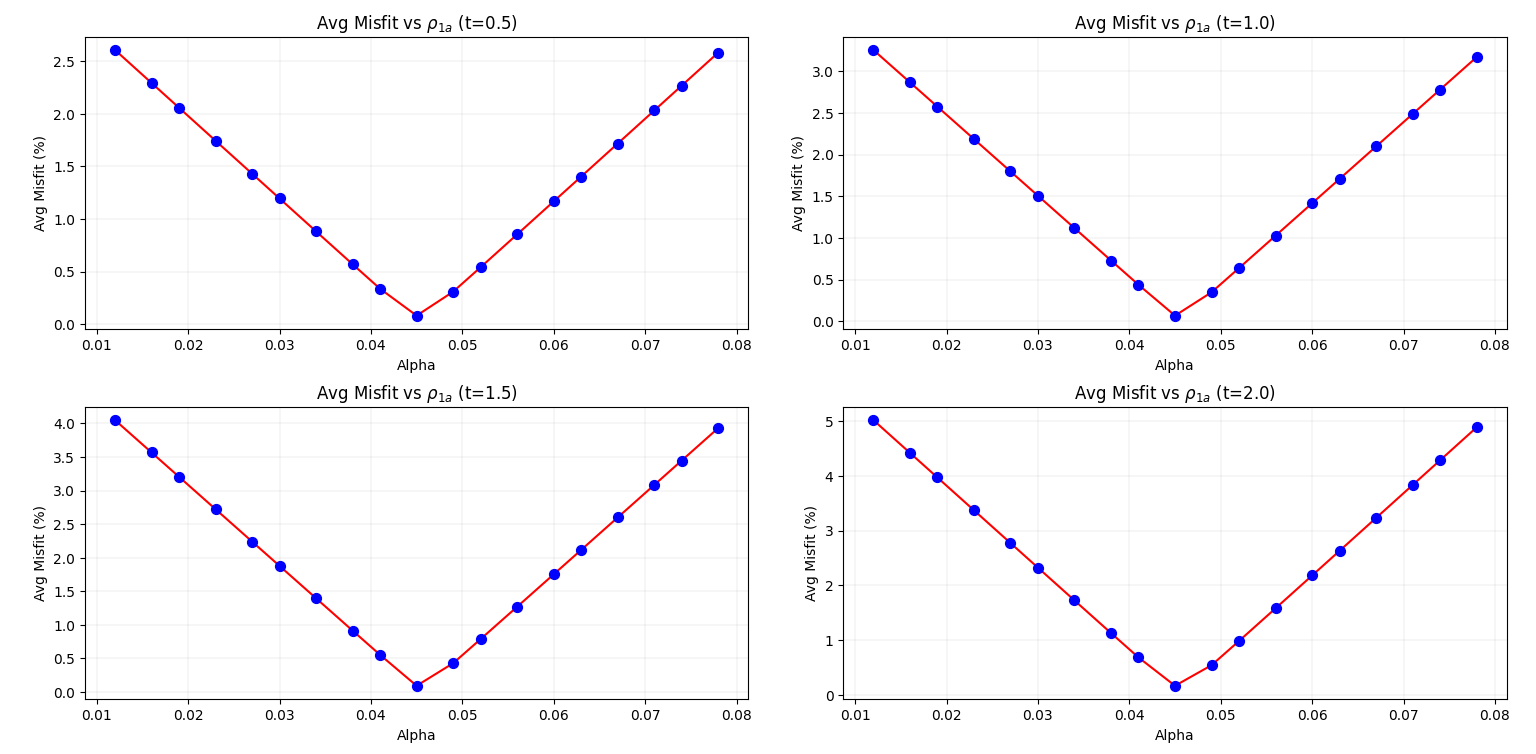
\includegraphics[width=0.8\linewidth]{Misfits across range/case 1 new.png}
     }
    \caption{Misfit across a large parameter range; linear perturbations with gravitational collapse}
    \label{Figure 7}
\end{figure}

\begin{figure}[H]
     \centering
     \makebox[\textwidth][c]{%
     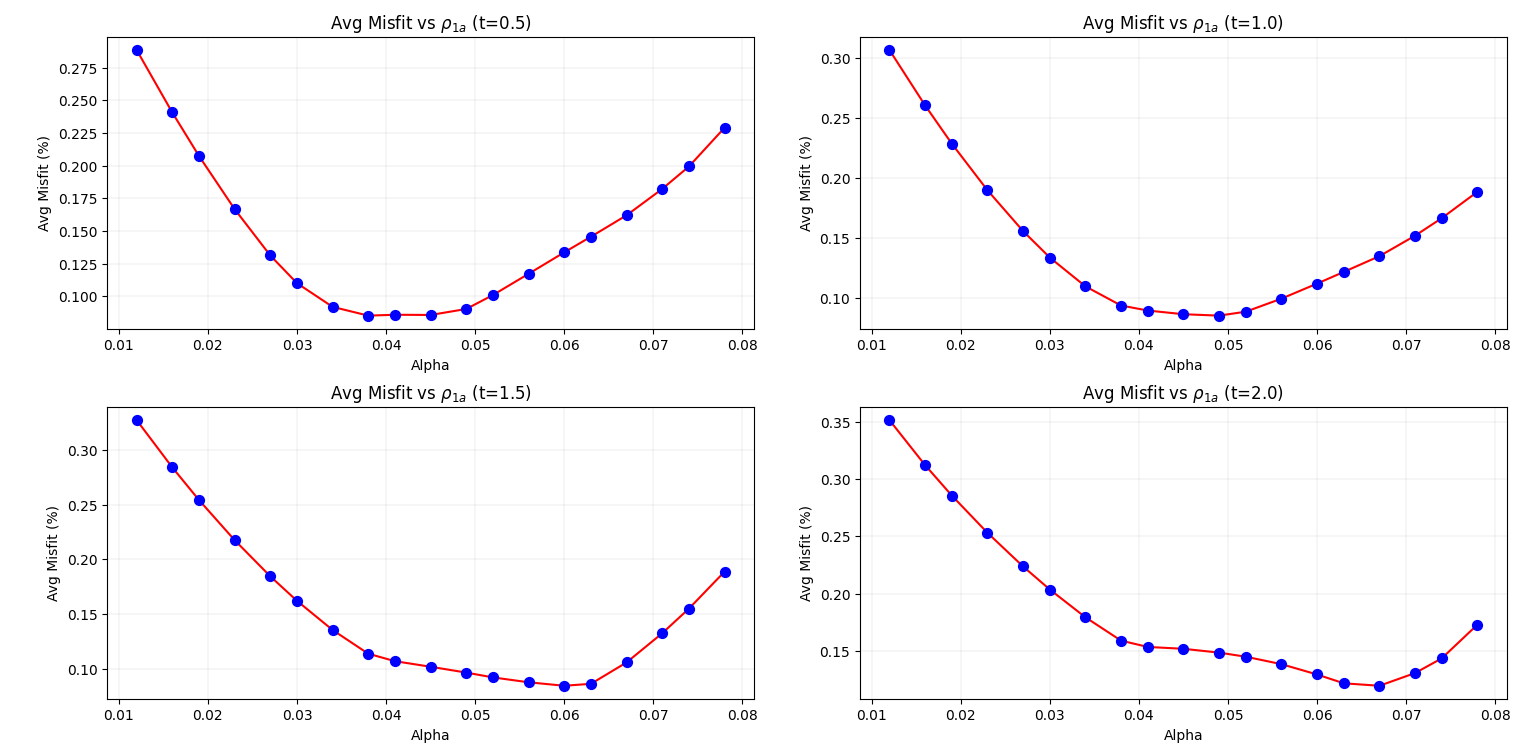
\includegraphics[width=0.8\linewidth]{Misfits across range/Case 3 new.png}
     }
    \caption{Misfit across a large parameter range; linear perturbations with no gravitational collapse}
    \label{Figure 8}
\end{figure}

\begin{figure}[H]
     \centering
     \makebox[\textwidth][c]{%
     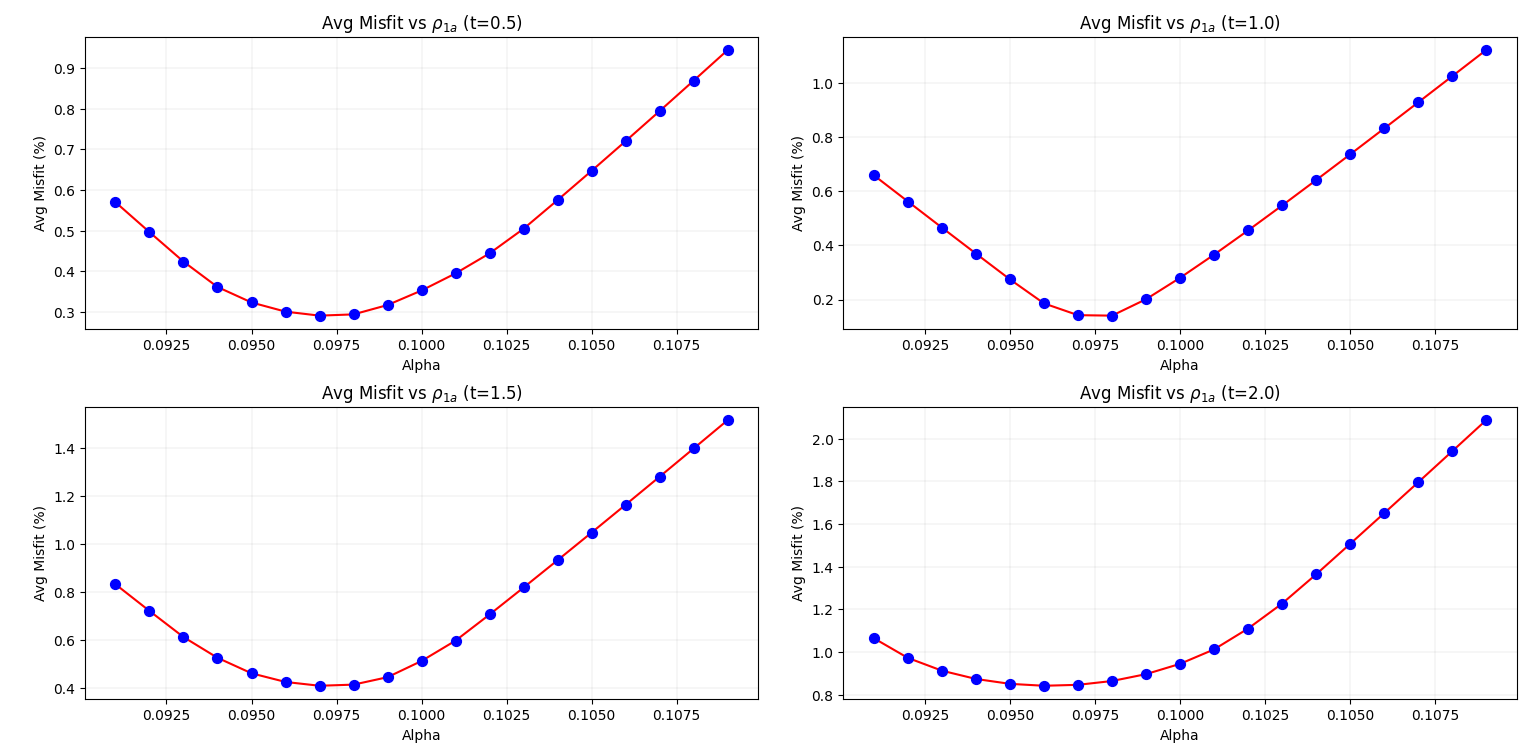
\includegraphics[width=0.8\linewidth]{Misfits across range/mixed case 1 and 2 new.png}
     }
    \caption{Misfit across a small parameter range; linear and non-linear perturbations with gravitational collapse}
    \label{Figure 9}
\end{figure}

\subsection{Performance across a large \texorpdfstring{$\rho_{1a}$ range}{rho1a range}}

One of the limitations of our framework is that it does not learn the solutions of a large range of parameters well, as can be shown in \autoref{Figure 7} for linear perturbations. The model is trained in a similar way as \autoref{Figure 1}, and tested on 20 different values in the same range. Our model compromises on a midway solution, instead of perfectly capturing the dependence of $\rho_{1a}$ on the amplitudes of density and velocity, especially near regions of high gravitational collapse. Such behaviour is not strongly seen when gravitational collapse does not occur, as can be seen in \autoref{Figure 8}, although there is a slight increase in error as we move towards high perturbation values. One interesting observation is that on reducing the parameter space, the errors can be reduced heavily, as can be seen in \autoref{Figure 9}, where instead of the range of \autoref{Figure 1}, we use a smaller range from $0.09$ to $0.11$. To strengthen our claim, we purposely take a range near the transition region, where the physics changes rapidly.

\section{Summary and Conclusions}

We develop a PINN based model for parameter learning of initial perturbation strength for efficient surrogate modelling of self-gravitating molecular clouds across wide parameter spaces. Improved computational speed in
modelling such flows could profoundly impact our understanding of star formation, which couples processes operating across a vast range of scales, from the diameter of our Galaxy down to the molecular mean free path that sets the thickness of shocks.
Our overall result is that the model is capable of learning the dependence of $\rho_{1a}$ on the PDE solutions, thus enabling surrogate modelling of self-gravitating molecular clouds.
The source code for GRINN is available on the GitHub software repository at

\section{Acknowledgements}

I would like to express my gratitude to Dr. Sayantan Auddy for his support and guidance throughout the project. His mentorship has allowed me to gain significant experience in the applications of Machine Learning in Astrophysics Research.
I would also like to thank Kaggle for providing 30 hours of GPU access per week to all users for free. This access enabled me to run hundreds of tests in a efficient manner, ranging from different hypotheses, model architectures, training loops and other optimisation techniques.

\printbibliography
\end{document}